\documentclass[tikz, border=2mm]{standalone}
\usepackage{tikz}


\begin{document}

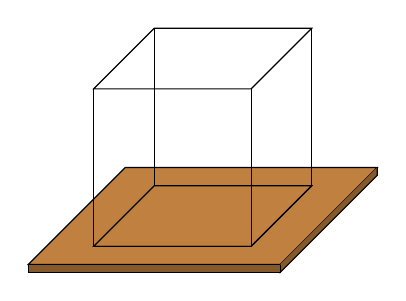
\begin{tikzpicture}[scale=2]

\draw [fill=brown] (-.3,0,-.3) -- (1.3,0,-.3) -- (1.3,0,1.3) -- (-.3,0,1.3) -- cycle;
\draw [fill=brown!70!black] (1.3,0,-.3) -- (1.3,-.05,-.3) -- (1.3,-.05,1.3) -- (1.3,0,1.3);
\draw [fill=brown!70!black] (1.3,0,1.3) -- (1.3,-.05,1.3) -- (-.3,-.05,1.3) -- (-.3,0,1.3);



\draw (0,0,0) -- (1,0,0) -- (1,0,1) -- (0,0,1) -- cycle;
\draw (0,1,0) -- (1,1,0) -- (1,1,1) -- (0,1,1) -- cycle;

\draw (0,0,0) -- (0,1,0);



% \fill [blue!70] (0,.25,0) -- (1,.25,0) -- (1,.25,1) -- (0,.25,1) -- cycle;
% \fill [blue!80] (0,0,1) -- (1,0,1) -- (1,.25,1) -- (0,.25,1) -- cycle;
% \fill [blue!80] (1,0,0) -- (1,0,1) -- (1,.25,1) -- (1,.25,0) -- cycle;

\draw (1,0,1) -- (1,1,1);
\draw (1,0,0) -- (1,1,0);
\draw (0,0,1) -- (0,1,1);
\draw (1,0,0) -- (1,0,1) -- (0,0,1);

\end{tikzpicture}

\end{document}

